%Version 2.1 April 2023
% See section 11 of the User Manual for version history
%
%%%%%%%%%%%%%%%%%%%%%%%%%%%%%%%%%%%%%%%%%%%%%%%%%%%%%%%%%%%%%%%%%%%%%%
%%                                                                 %%
%% Please do not use \input{...} to include other tex files.       %%
%% Submit your LaTeX manuscript as one .tex document.              %%
%%                                                                 %%
%% All additional figures and files should be attached             %%
%% separately and not embedded in the \TeX\ document itself.       %%
%%                                                                 %%
%%%%%%%%%%%%%%%%%%%%%%%%%%%%%%%%%%%%%%%%%%%%%%%%%%%%%%%%%%%%%%%%%%%%%

\documentclass[sn-vancouver,Numbered,lineno,pdflatex]{sn-jnl}

%%%% Standard Packages
%%<additional latex packages if required can be included here>

\usepackage{graphicx}%
\usepackage{multirow}%
\usepackage{amsmath,amssymb,amsfonts}%
\usepackage{amsthm}%
\usepackage{mathrsfs}%
\usepackage[title]{appendix}%
\usepackage{xcolor}%
\usepackage{textcomp}%
\usepackage{manyfoot}%
\usepackage{booktabs}%
\usepackage{algorithm}%
\usepackage{algorithmicx}%
\usepackage{algpseudocode}%
\usepackage{listings}%
%%%%

%%%%%=============================================================================%%%%
%%%%  Remarks: This template is provided to aid authors with the preparation
%%%%  of original research articles intended for submission to journals published
%%%%  by Springer Nature. The guidance has been prepared in partnership with
%%%%  production teams to conform to Springer Nature technical requirements.
%%%%  Editorial and presentation requirements differ among journal portfolios and
%%%%  research disciplines. You may find sections in this template are irrelevant
%%%%  to your work and are empowered to omit any such section if allowed by the
%%%%  journal you intend to submit to. The submission guidelines and policies
%%%%  of the journal take precedence. A detailed User Manual is available in the
%%%%  template package for technical guidance.
%%%%%=============================================================================%%%%

\usepackage{natbib}
\usepackage{hyperref}
\usepackage[utf8]{inputenc}
\usepackage{capt-of}
\usepackage{booktabs}
\usepackage{amssymb}
\usepackage{threeparttable}
\usepackage{float}
%\floatplacement{figure}{H}
%\floatplacement{table}{H}
\usepackage{lipsum,caption}
\geometry{
  a4paper,
  left=1in,
  right=1in,
  top=1in,
  bottom=1in,
  includeheadfoot
}
\usepackage{setspace}
%\usepackage{lineno}
%\linenumbers
\usepackage{siunitx}
\sisetup{
  mode = match,
  propagate-math-font = true,
  reset-math-version = false,
  reset-text-family = false,
  reset-text-series = false,
  reset-text-shape = false,
  text-family-to-math = true,
  text-series-to-math = true
}
\doublespacing
% Disable explicit page breaks in LaTeX
\let\clearpage\relax



\raggedbottom




% tightlist command for lists without linebreak
\providecommand{\tightlist}{%
  \setlength{\itemsep}{0pt}\setlength{\parskip}{0pt}}





\begin{document}


\title[High-Dimensional Propensity Score]{Understanding the role of
different proxy selection methods in High-Dimensional Propensity Score
Analysis}

%%=============================================================%%
%% Prefix	-> \pfx{Dr}
%% GivenName	-> \fnm{Joergen W.}
%% Particle	-> \spfx{van der} -> surname prefix
%% FamilyName	-> \sur{Ploeg}
%% Suffix	-> \sfx{IV}
%% NatureName	-> \tanm{Poet Laureate} -> Title after name
%% Degrees	-> \dgr{MSc, PhD}
%% \author*[1,2]{\pfx{Dr} \fnm{Joergen W.} \spfx{van der} \sur{Ploeg} \sfx{IV} \tanm{Poet Laureate}
%%                 \dgr{MSc, PhD}}\email{iauthor@gmail.com}
%%=============================================================%%

\author*[1,2]{\pfx{Dr.} \fnm{Mohammad Ehsanul} \sur{Karim} \dgr{MSc,
PhD}}\email{\href{mailto:ehsan.karim@ubc.ca}{\nolinkurl{ehsan.karim@ubc.ca}}}

\author[3]{\fnm{Yang} \sur{Lei} }



  \affil*[1]{\orgdiv{School of Population and Public
Health}, \orgname{University of British
Columbia}, \orgaddress{\city{Vancouver}, \country{Canada}, \postcode{V6T
1Z3}, \state{BC}, \street{2206 East Mall}}}
  \affil[2]{\orgname{St.~Paul's
Hospital}, \orgaddress{\city{Vancouver}, \country{Canada}, \postcode{V6Z
1Y6}, \state{BC}, \street{588 - 1081 Burrard Street}}}
  \affil[3]{\orgdiv{Department of Statistics}, \orgname{University of
British
Columbia}, \orgaddress{\city{Vancouver}, \country{Canada}, \postcode{V6T
1Z4}, \state{BC}, \street{Room 3182 Earth Sciences Building, 2207 Main
Mall}}}

\abstract{\textbf{Purpose}: \textbf{Methods:} \textbf{Results:}
\textbf{Conclusion:}}

\keywords{Machine learning, Propensity score, Deep learning, Causal
inference}


\pacs[JEL Classification]{C18}
\pacs[MSC Classification]{92D30, 62P10}

\maketitle

\section{Background}\label{background}

\textbf{Aim}: The aim of this research is to systematically evaluate and
compare different proxy selection methods within the context of
high-dimensional propensity score (hdPS) analysis. Specifically, the
study focuses on assessing how these methods, including alternative
variable selection approaches, perform in selecting proxy variables for
confounding adjustment compared to the traditional Bross method within
the hdPS framework. We seek to determine whether these alternative
methods offer superior performance in estimating treatment effects
compared to the default Bross formula.

\section{Methods}\label{methods}

\subsection*{Data and Simulation}\label{data-and-simulation}
\addcontentsline{toc}{subsection}{Data and Simulation}

\textbf{Motivating Example}: To explore the relationship between obesity
and the risk of diabetes, we revisited this association using data from
three cycles of the National Health and Nutrition Examination Survey
(NHANES) covering the years 2013-2014, 2015-2016, and 2017-2018
\citep{karim2024high}. This analysis was informed by a thorough review
of the existing literature
\citep{saydah2014trends, liu2013association, kabadi2012joint, ostchega2012abdominal}.
To identify relevant covariates, we constructed a causal diagram based
on established causal inference principles \citep{greenland1999causal}.
The covariates included in our analysis were carefully selected and
categorized into Demographic, Behavioral, Health History,
Access-related, and Laboratory variables \citep{karim2024high}. While
most of these variables were binary or categorical, the Laboratory
variables were continuous.

\textbf{Plasmode simulation}: To rigorously assess the performance of
the methods under consideration, we employed a plasmode simulation
framework, which is particularly well-suited for reflecting real-world
data structures and complexities \citep{franklin2014plasmode}. This
approach was modeled after the analytic dataset derived from NHANES and
involved resampling from the observed covariates and exposure
information (i.e., obesity) without altering them. By mirroring key
aspects of an actual epidemiological study, this simulation framework
offers a significant advantage over traditional Monte Carlo simulations,
which often rely on idealized assumptions.

\textbf{Simulation scenarios under consideration}: Our plasmode
simulation was conducted over 500 iterations. For the base simulation
scenario, we set the prevalence of exposure (obesity) and the event rate
(diabetes) at 30\%, with a true odds ratio (OR) parameter of 1,
corresponding to a risk difference (RD) of 0. Each simulated dataset had
a sample size of 3,000 participants. The description of other scenarios
under consideration is provided in Table \ref{table:scenarios}.

\begin{table}[ht]
\centering
\caption{Overview of Plasmode Simulation Scenarios Reflecting Varying Exposure and Outcome Prevalences Based on National Health and Nutrition Examination Survey (NHANES) Data Cycles (2013-2018)}
\label{table:scenarios}
\begin{tabular}{lcccc}
  \toprule
  \textbf{Plasmode Simulation Scenario} & \textbf{Exposure} & \textbf{Outcome} & \textbf{True} & \textbf{Sample}\\
  \textbf{} & \textbf{Prevalence} & \textbf{Prevalence} & \textbf{Odds Ratio} & \textbf{Size}\\
  \midrule
  (i) Frequent Exposure and Outcome (Base) & 30\% & 30\% & 1 & 3,000 \\
  (ii) Rare Exposure and Frequent Outcome & 5\% & 30\% & 1 & 3,000 \\
  (iii) Frequent Exposure and Rare Outcome & 30\% & 5\% & 1 & 3,000 \\
  \bottomrule
\end{tabular}
\end{table}

\textbf{True Data Generating Mechanism Used in Plasmode Simulation}: The
primary goal of this study is to evaluate various variable selection
methods under realistic conditions. To achieve this, we formulated the
outcome data based on a specific model specification that incorporates
both exposure and covariates, including investigator-specified and proxy
variables. The model specification consists of three key components:

\begin{enumerate}
\def\labelenumi{\arabic{enumi}.}
\item
  \emph{Investigator-Specified Covariates}: We retained the original
  investigator-specified covariates, which were either binary or
  categorical, reflecting how real-world studies typically operate.
\item
  \emph{Transformation of Laboratory Variables}: In real-world studies,
  it is common for analysts to lack precise knowledge of the true model
  specification. To simulate this uncertainty, we transformed the
  continuous laboratory variables using complex functions such as
  logarithmic, exponential, square root, polynomial transformations, and
  interactions. This reflects the challenges analysts face in correctly
  specifying models when dealing with continuous data.
\item
  \emph{Inclusion of Proxy Variables}: Real-world studies often deal
  with unmeasured confounding, which researchers attempt to mitigate by
  adding proxy variables. However, when a large number of proxies are
  added, some may act as noise variables, contributing little to the
  analysis. To simulate this, we selected only those binary proxy
  covariates (referred to as recurrence covariates in hdPS terminology)
  that had a relative risk (RR) of less than 0.8 or greater than 1.2
  concerning the outcome. Out of 143 proxy covariates, 94 met this
  criterion and were included in calculating a simple comorbidity burden
  measure. The remaining 49 covariates were excluded from this
  calculation and considered noise. This comorbidity burden measure was
  then incorporated into our model specification for generating the
  plasmode data.
\end{enumerate}

\textbf{Performance Measures}: From this simulation, we derived several
performance metrics to evaluate the effectiveness of the methods under
consideration: (1) bias, (2) average model standard error (SE; the
average of estimated SEs obtained from a model over repeated samples),
(3) empirical SE (the standard deviation of estimated treatment effects
across repeated samples), (4) mean squared error (MSE), (5) coverage
probability of 95\% confidence intervals, (6) bias-corrected coverage,
and (7) Zip plot \citep{morris2019using, white2023check}.

\subsection*{Estimators under
consideration}\label{estimators-under-consideration}
\addcontentsline{toc}{subsection}{Estimators under consideration}

The comparison between the data generation process and the analysis
process reveals two key differences: (i) The data generation used
transformed laboratory variables, whereas the analysis was conducted
using only the original laboratory variables. (ii) The data generation
employed a simple sum of selected proxy variables (sum of 94 proxy
covariates), while the analysis included all proxy variables (143 binary
proxies), with 49 of these acting as noise variables. These differences
help us assess how the proxy variable selection methods handle model
misspecification and the presence of noise variables.

\begin{enumerate}
\def\labelenumi{\arabic{enumi}.}
\item
  \textbf{Kitchen sink model}: This is a base model for comparison,
  where no variable selection approaches were used. All
  investigator-selected features and all proxy variables were used to
  model \citep{karim2018can}.
\item
  \textbf{Bross formula}: The Bross formula is a statistical method used
  to calculate the bias introduced by not adjusting for a covariate
  \citep{bross1966spurious}. In hdPS analysis, this formula was
  originally applied to each proxy variable to measure and rank the
  potential bias if the covariate were not adjusted for. In our
  analysis, the 100 proxies with the highest bias rankings are selected
  for further modeling \citep{schneeweiss2009high, wyss2018erratum}.
\item
  \textbf{Least Absolute Shrinkage and Selection Operator (LASSO)}:
  LASSO is a variable selection technique that limits the number of
  variables by adding a penalty term to the regression model.
  Cross-validation (CV) is used in LASSO to identify variables with
  non-zero coefficients in the best model by optimizing the penalty
  value
  \citep{franklin2015regularized, schneeweiss2017variable, karim2018can}.
\item
  \textbf{Hybrid of hdPS and LASSO}: Instead of relying solely on LASSO
  for variable selection, a hybrid approach combines the Bross formula
  and LASSO. First, hdPS variables are selected using the hdPS algorithm
  (e.g., the top 100), and then LASSO is applied to further refine the
  selection \citep{karim2018can, franklin2015regularized}.
\item
  \textbf{Elasticnet}: Elastic Net is an extension of LASSO that
  includes an additional penalty term to handle multicollinearity by
  grouping correlated features and selecting the most representative
  ones \citep{karim2018can}.
\item
  \textbf{Random Forest}: The Random Forest (RF) algorithm is an
  ensemble learning method that constructs multiple decision trees to
  perform classification \citep{breiman2001random}. It calculates the
  importance of each proxy variable based on the decrease in impurity or
  Gini importance, providing a ranking of the proxies. The top 100
  variables from this ranking are manually selected for further modeling
  \citep{schneeweiss2017variable}.
\item
  \textbf{XGBoost}: XGBoost is a gradient boosting algorithm used to
  optimize machine learning models \citep{chen2016xgboost}. It builds
  decision trees that make splits based on maximum impurity reduction,
  and it assigns an importance score to each proxy variable by
  calculating the mean decrease in impurity
  \citep{xiao2024interpretable}.
\item
  \textbf{Stepwise}: Stepwise selection is a progressive feature
  selection method that can proceed in two directions---forward or
  backward---based on the maximum adjusted R-squared. We have
  implemented two versions: (a) Forward selection (FS) starts with an
  initial model (e.g., including all investigator-selected features) and
  adds proxies to the model one at a time. (b) Backward elimination (BE)
  starts with a full model (e.g., all investigator-selected features and
  all proxy variables) and removes features one at a time based on their
  contribution to the model.
\item
  \textbf{Genetic algorithm (GA)}: GA is an evolutionary algorithm
  inspired by the theory of natural selection
  \citep{holland1975adaptation}. It operates by evolving offspring from
  a population of the fittest individuals over several generations,
  evaluating and selecting the best combination of features or variables
  that maximize prediction accuracy.
\end{enumerate}

\section{Results}\label{results}

The results for each method under the different scenarios are summarized
below. See Figures \ref{fig:bias-comparison} and
\ref{fig:Coverage-comparison} for an overview of the performance in
terms of bias and coverage, respectively.

\begin{enumerate}
\def\labelenumi{(\roman{enumi})}
\tightlist
\item
  \textbf{Frequent Exposure and Outcome (base) scenario}:
\end{enumerate}

\begin{enumerate}
\def\labelenumi{\arabic{enumi}.}
\item
  \emph{Bias}: The kitchen sink model, which includes all variables
  without selection, exhibited the smallest bias (0.0002). In contrast,
  the Genetic Algorithm (GA) showed the highest bias (0.0287). Among the
  other methods, Bross (-0.0001), Hybrid (0.0016), and Elasticnet
  (0.0036) demonstrated low bias, indicating that these methods provide
  estimates closer to the true effect. XGBoost (0.0074) and Random
  Forest (RF) (0.0034) had slightly higher bias but remained within
  acceptable limits.
\item
  \emph{Coverage}: Most methods, including Hybrid, Forward, Backward,
  LASSO, and Elasticnet, achieved high coverage values around 98\(\%\),
  indicating well-calibrated confidence intervals. However, the GA
  method had significantly lower coverage (83.8\(\%\)), suggesting that
  its confidence intervals might be too narrow or biased, potentially
  missing the true effect. Given the bias in the GA method's results, we
  also calculated bias-eliminated coverage. This adjustment improved
  GA's coverage to 96\(\%\), but it still remained lower than that of
  the other methods.
\item
  \emph{Mean Squared Error (MSE)}: XGBoost achieved the lowest MSE
  (0.0006), indicating it as the most accurate method overall.
  Conversely, the GA method had the highest MSE (0.0016), reflecting its
  higher bias and variability. The kitchen sink model (0.0009), Bross
  (0.0008), Hybrid (0.0008), and Elasticnet (0.0009) all had relatively
  similar and moderate MSE values.
\item
  \emph{Standard Error (SE)}: The lowest Empirical SE was observed with
  XGBoost (0.0229), indicating high precision in its estimates. The
  kitchen sink model had the highest Empirical SE (0.0305), suggesting
  greater variability. Other methods such as GA (0.0274), Hybrid
  (0.0278), and Bross (0.0287) exhibited moderate variability, while
  LASSO (0.0299) and Elasticnet (0.0294) had slightly higher
  variability. Similarly, XGBoost also showed the lowest Model-based SE
  (0.0268), consistent with its low Empirical SE and indicating high
  precision. The kitchen sink model had the highest Model-based SE
  (0.0333), suggesting less precision in its estimates.
\end{enumerate}

\textbf{(ii) Rare Exposure and Frequent Outcome}:

\begin{enumerate}
\def\labelenumi{\arabic{enumi}.}
\item
  \emph{Bias}: In this scenario, the kitchen sink model showed a
  relatively low bias (0.0025), but the Genetic Algorithm (GA) had the
  highest bias (0.0408), indicating a substantial deviation from the
  true effect. XGBoost (0.0259) also exhibited higher bias compared to
  other methods. On the other hand, Bross (0.0035), Hybrid (0.0049), and
  Elasticnet (0.0053) demonstrated moderate bias, while Random Forest
  (RF) (0.0127) and Forward Selection (0.0108) had slightly higher bias
  but remained within an acceptable range.
\item
  \emph{Coverage}: Most methods maintained high coverage levels, with
  XGBoost showing the highest coverage (96.2\(\%\)), suggesting that its
  confidence intervals were well-calibrated despite the higher bias. The
  GA method, however, had slightly lower coverage (92.2\(\%\)),
  indicating that its confidence intervals might be narrower,
  potentially excluding the true effect. Other methods such as RF,
  Forward, Backward, and Hybrid had coverage values around 95\(\%\),
  suggesting adequate interval calibration. To account for the bias in
  GA, bias-eliminated coverage was calculated, which improved the
  coverage for GA to 94.2\(\%\), still slightly lower than other
  methods.
\item
  \emph{Mean Squared Error (MSE)}: XGBoost and Hybrid methods both
  demonstrated the lowest MSE (0.0032), indicating that these methods
  were the most accurate in this scenario. The GA method, with a higher
  MSE (0.0043), reflected its substantial bias and variability. The
  kitchen sink model had an MSE of 0.0043, similar to GA, while other
  methods such as Bross, RF, and Elasticnet exhibited moderate MSE
  values, indicating reasonable accuracy.
\item
  \emph{Standard Error (SE)}: The lowest Empirical SE was observed with
  XGBoost (0.0507) and GA (0.0510), reflecting the high precision of
  these methods despite the higher bias. The kitchen sink model
  exhibited the highest Empirical SE (0.0656), indicating greater
  variability. Methods like Hybrid (0.0564), Bross (0.0595), and RF
  (0.0609) showed moderate variability, while Elasticnet (0.0597) and
  LASSO (0.0587) had slightly higher variability. In terms of
  Model-based SE, XGBoost (0.0531) and GA (0.0533) also showed low
  variability, while the kitchen sink model had the highest Model-based
  SE (0.0623), suggesting less precision in its estimates.
\end{enumerate}

\textbf{(iii) Frequent Exposure and Rare Outcome}:

\begin{enumerate}
\def\labelenumi{\arabic{enumi}.}
\item
  \emph{Bias}: In this scenario, the kitchen sink model exhibited a
  moderate negative bias (-0.0093), similar to the Bross method
  (-0.0088). The Genetic Algorithm (GA) showed a significantly higher
  bias (0.0362), indicating a substantial deviation from the true
  effect. Among other methods, XGBoost demonstrated the lowest bias
  (-0.0061), while methods like Hybrid (-0.0082), Forward (-0.0070), and
  Backward (-0.0070) had slightly higher but still moderate biases.
  Elasticnet and LASSO both had biases of -0.0079, reflecting slightly
  larger deviations compared to XGBoost but still within acceptable
  limits.
\item
  \emph{Coverage}: Most methods achieved good coverage, with XGBoost,
  Random Forest (RF), and Forward Selection each achieving a coverage
  rate of 95.4\(\%\), indicating well-calibrated confidence intervals.
  The GA method, however, had slightly lower coverage (91.8\(\%\)),
  indicating that its confidence intervals might be narrower,
  potentially excluding the true effect. Bross and the kitchen sink
  model had slightly lower coverage values of 93.8\(\%\) and 93.4\(\%\),
  respectively. After accounting for bias, the bias-eliminated coverage
  for most methods, except GA, remained high, with values ranging from
  98.4\(\%\) to 99.0\(\%\), indicating that most methods effectively
  adjusted for bias in their coverage estimates. GA's bias-eliminated
  coverage was lower at 93.4\(\%\), reflecting its higher inherent bias.
\item
  \emph{Mean Squared Error (MSE)}: XGBoost exhibited the lowest MSE
  (0.0003), indicating it as the most accurate method overall in this
  scenario. GA had the highest MSE (0.0040), reflecting its substantial
  bias and variability. The kitchen sink model (0.0005), Bross (0.0005),
  and other methods like Hybrid (0.0004) and Elasticnet (0.0005) all had
  relatively similar MSE values, indicating moderate accuracy.
\item
  \emph{Standard Error (SE)}: The lowest Empirical SE was observed with
  XGBoost (0.0152), reflecting high precision in its estimates. The GA
  method exhibited the highest Empirical SE (0.0523), indicating greater
  variability and less precision. Methods like Hybrid (0.0184), Forward
  (0.0187), and Elasticnet (0.0203) showed moderate variability, while
  Bross (0.0206) and the kitchen sink model (0.0212) had slightly higher
  variability. In terms of Model-based SE, XGBoost (0.0179) again showed
  the lowest variability, consistent with its low Empirical SE,
  indicating that it provided the most stable estimates. The kitchen
  sink model had a slightly higher Model-based SE (0.0219), indicating
  less precision in its estimates.
\end{enumerate}

\begin{figure}[th]

{\centering 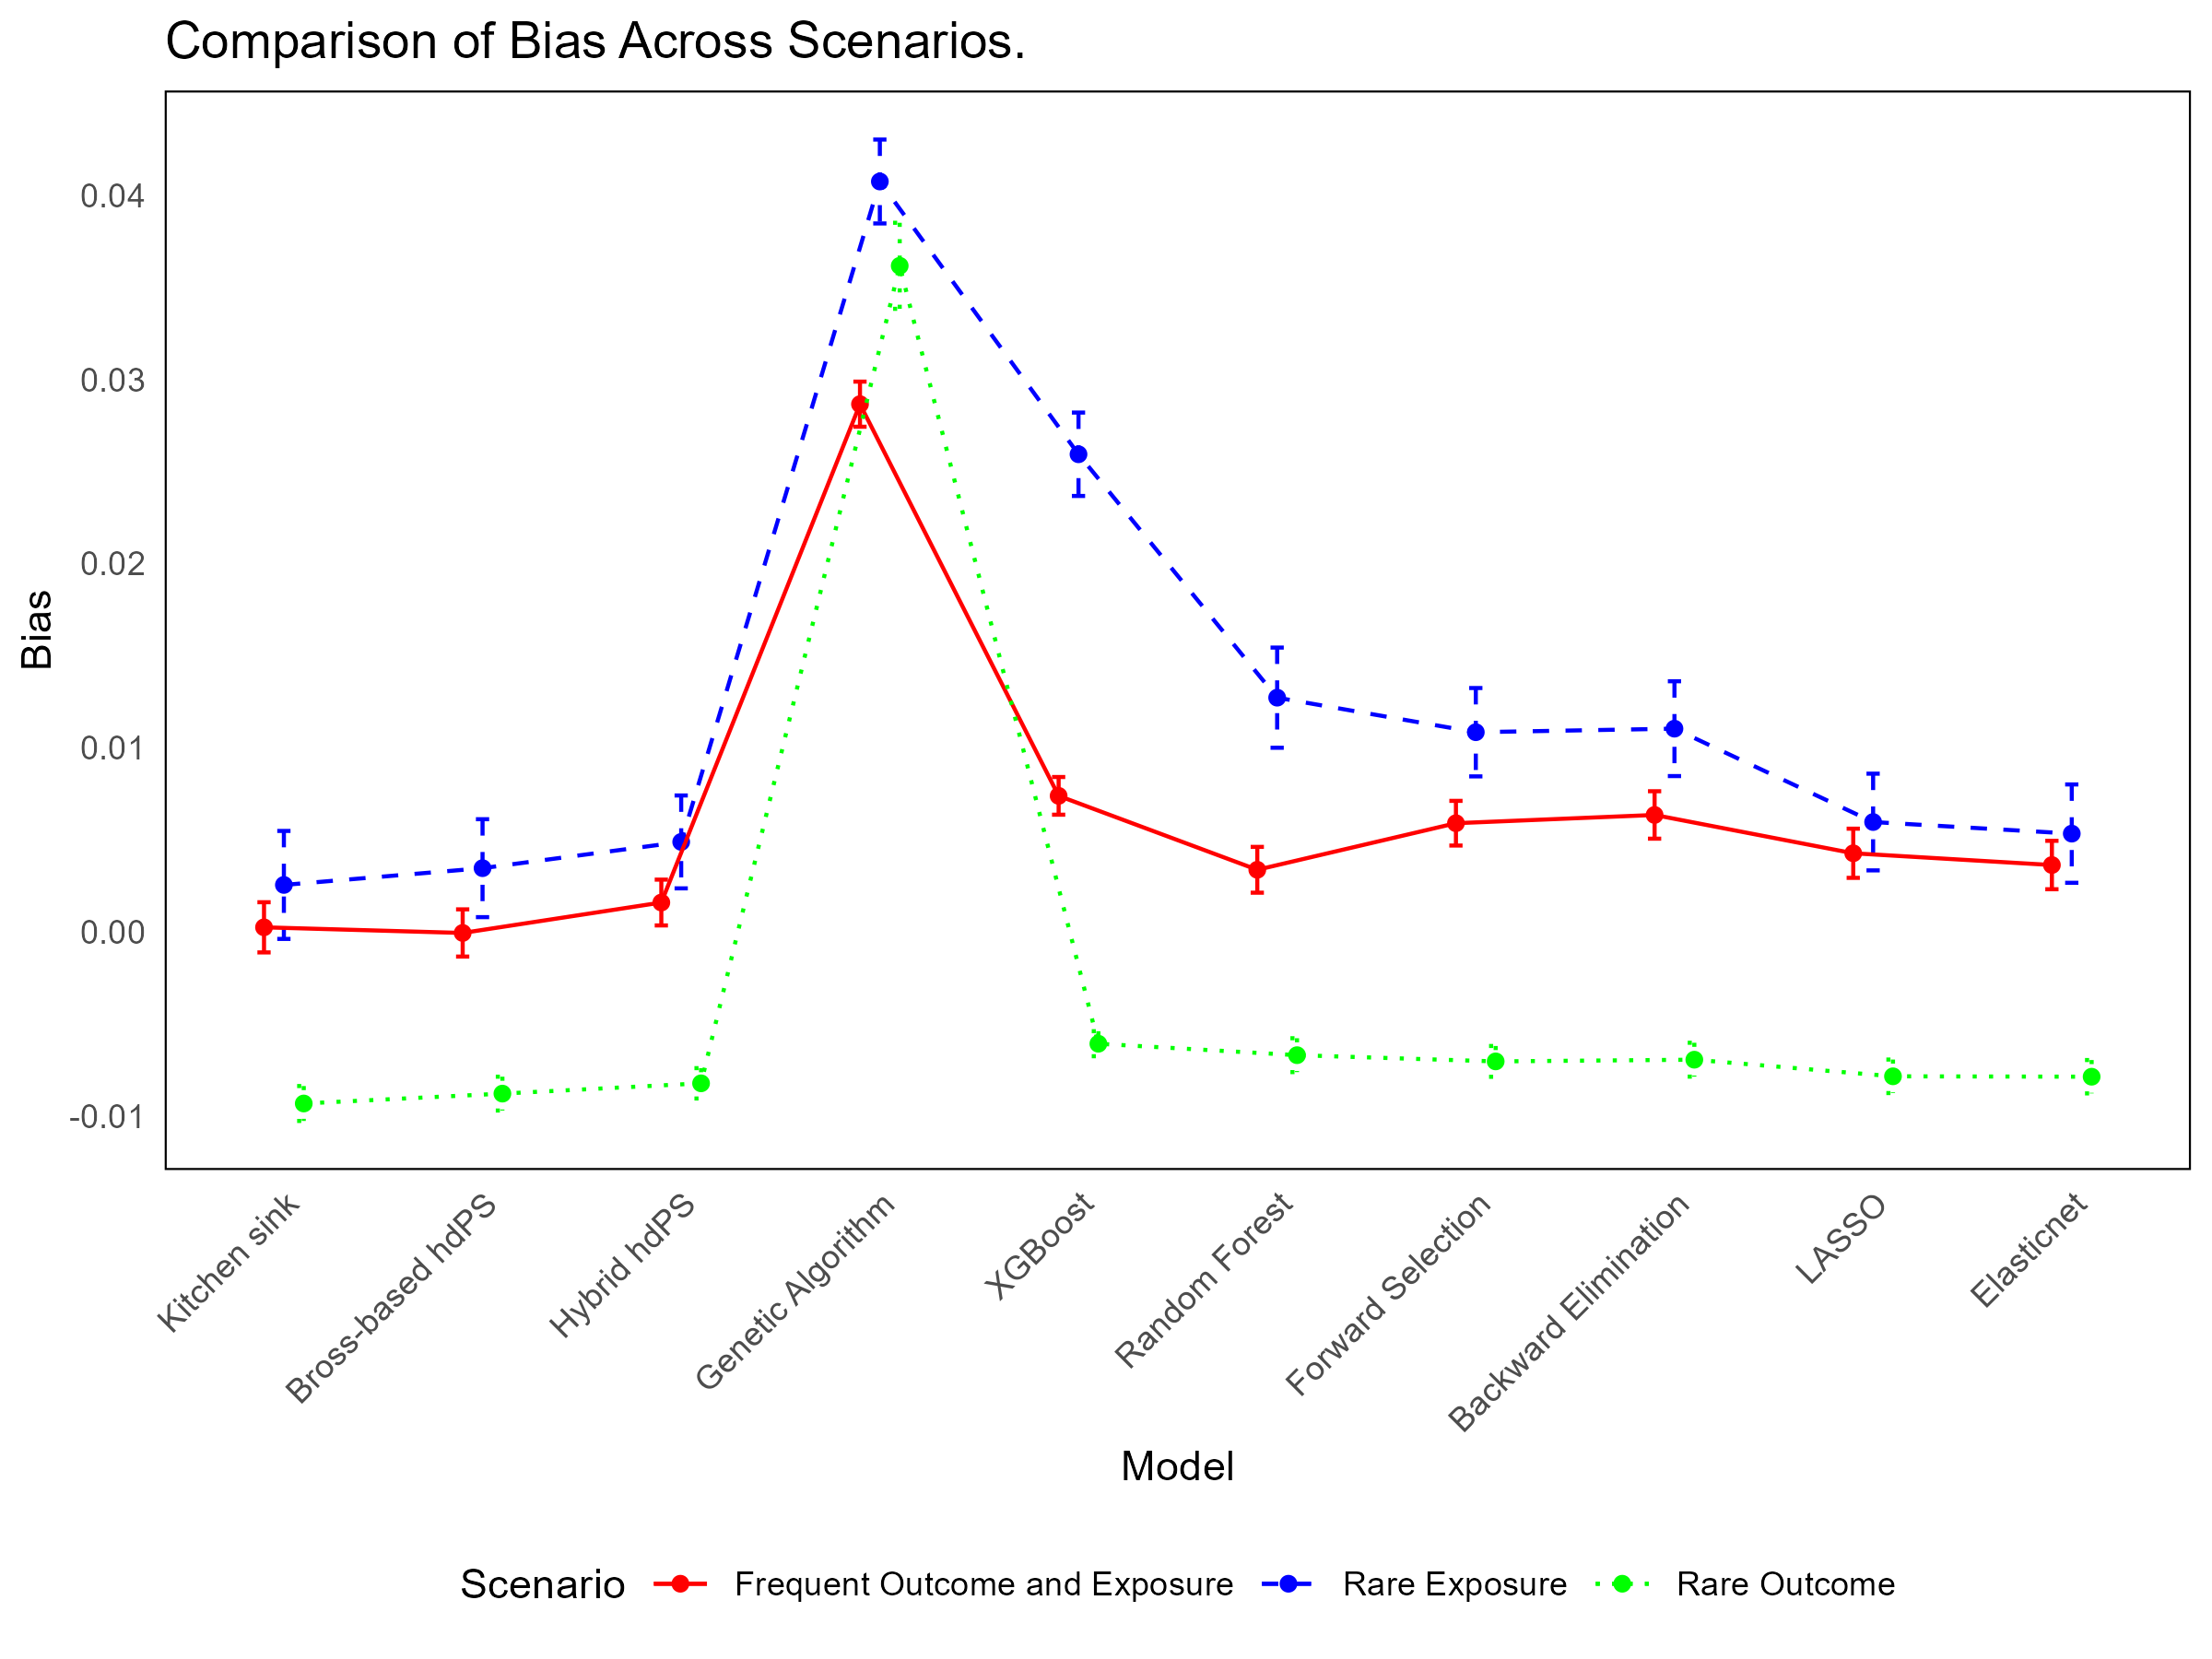
\includegraphics[width=1\linewidth,]{figures/metric_comparison_Bias} 

}

\caption{Comparison of Bias Across Different Methods in hdPS Analysis\label{fig:bias-comparison}}\label{fig:unnamed-chunk-1}
\end{figure}

\begin{figure}[th]

{\centering 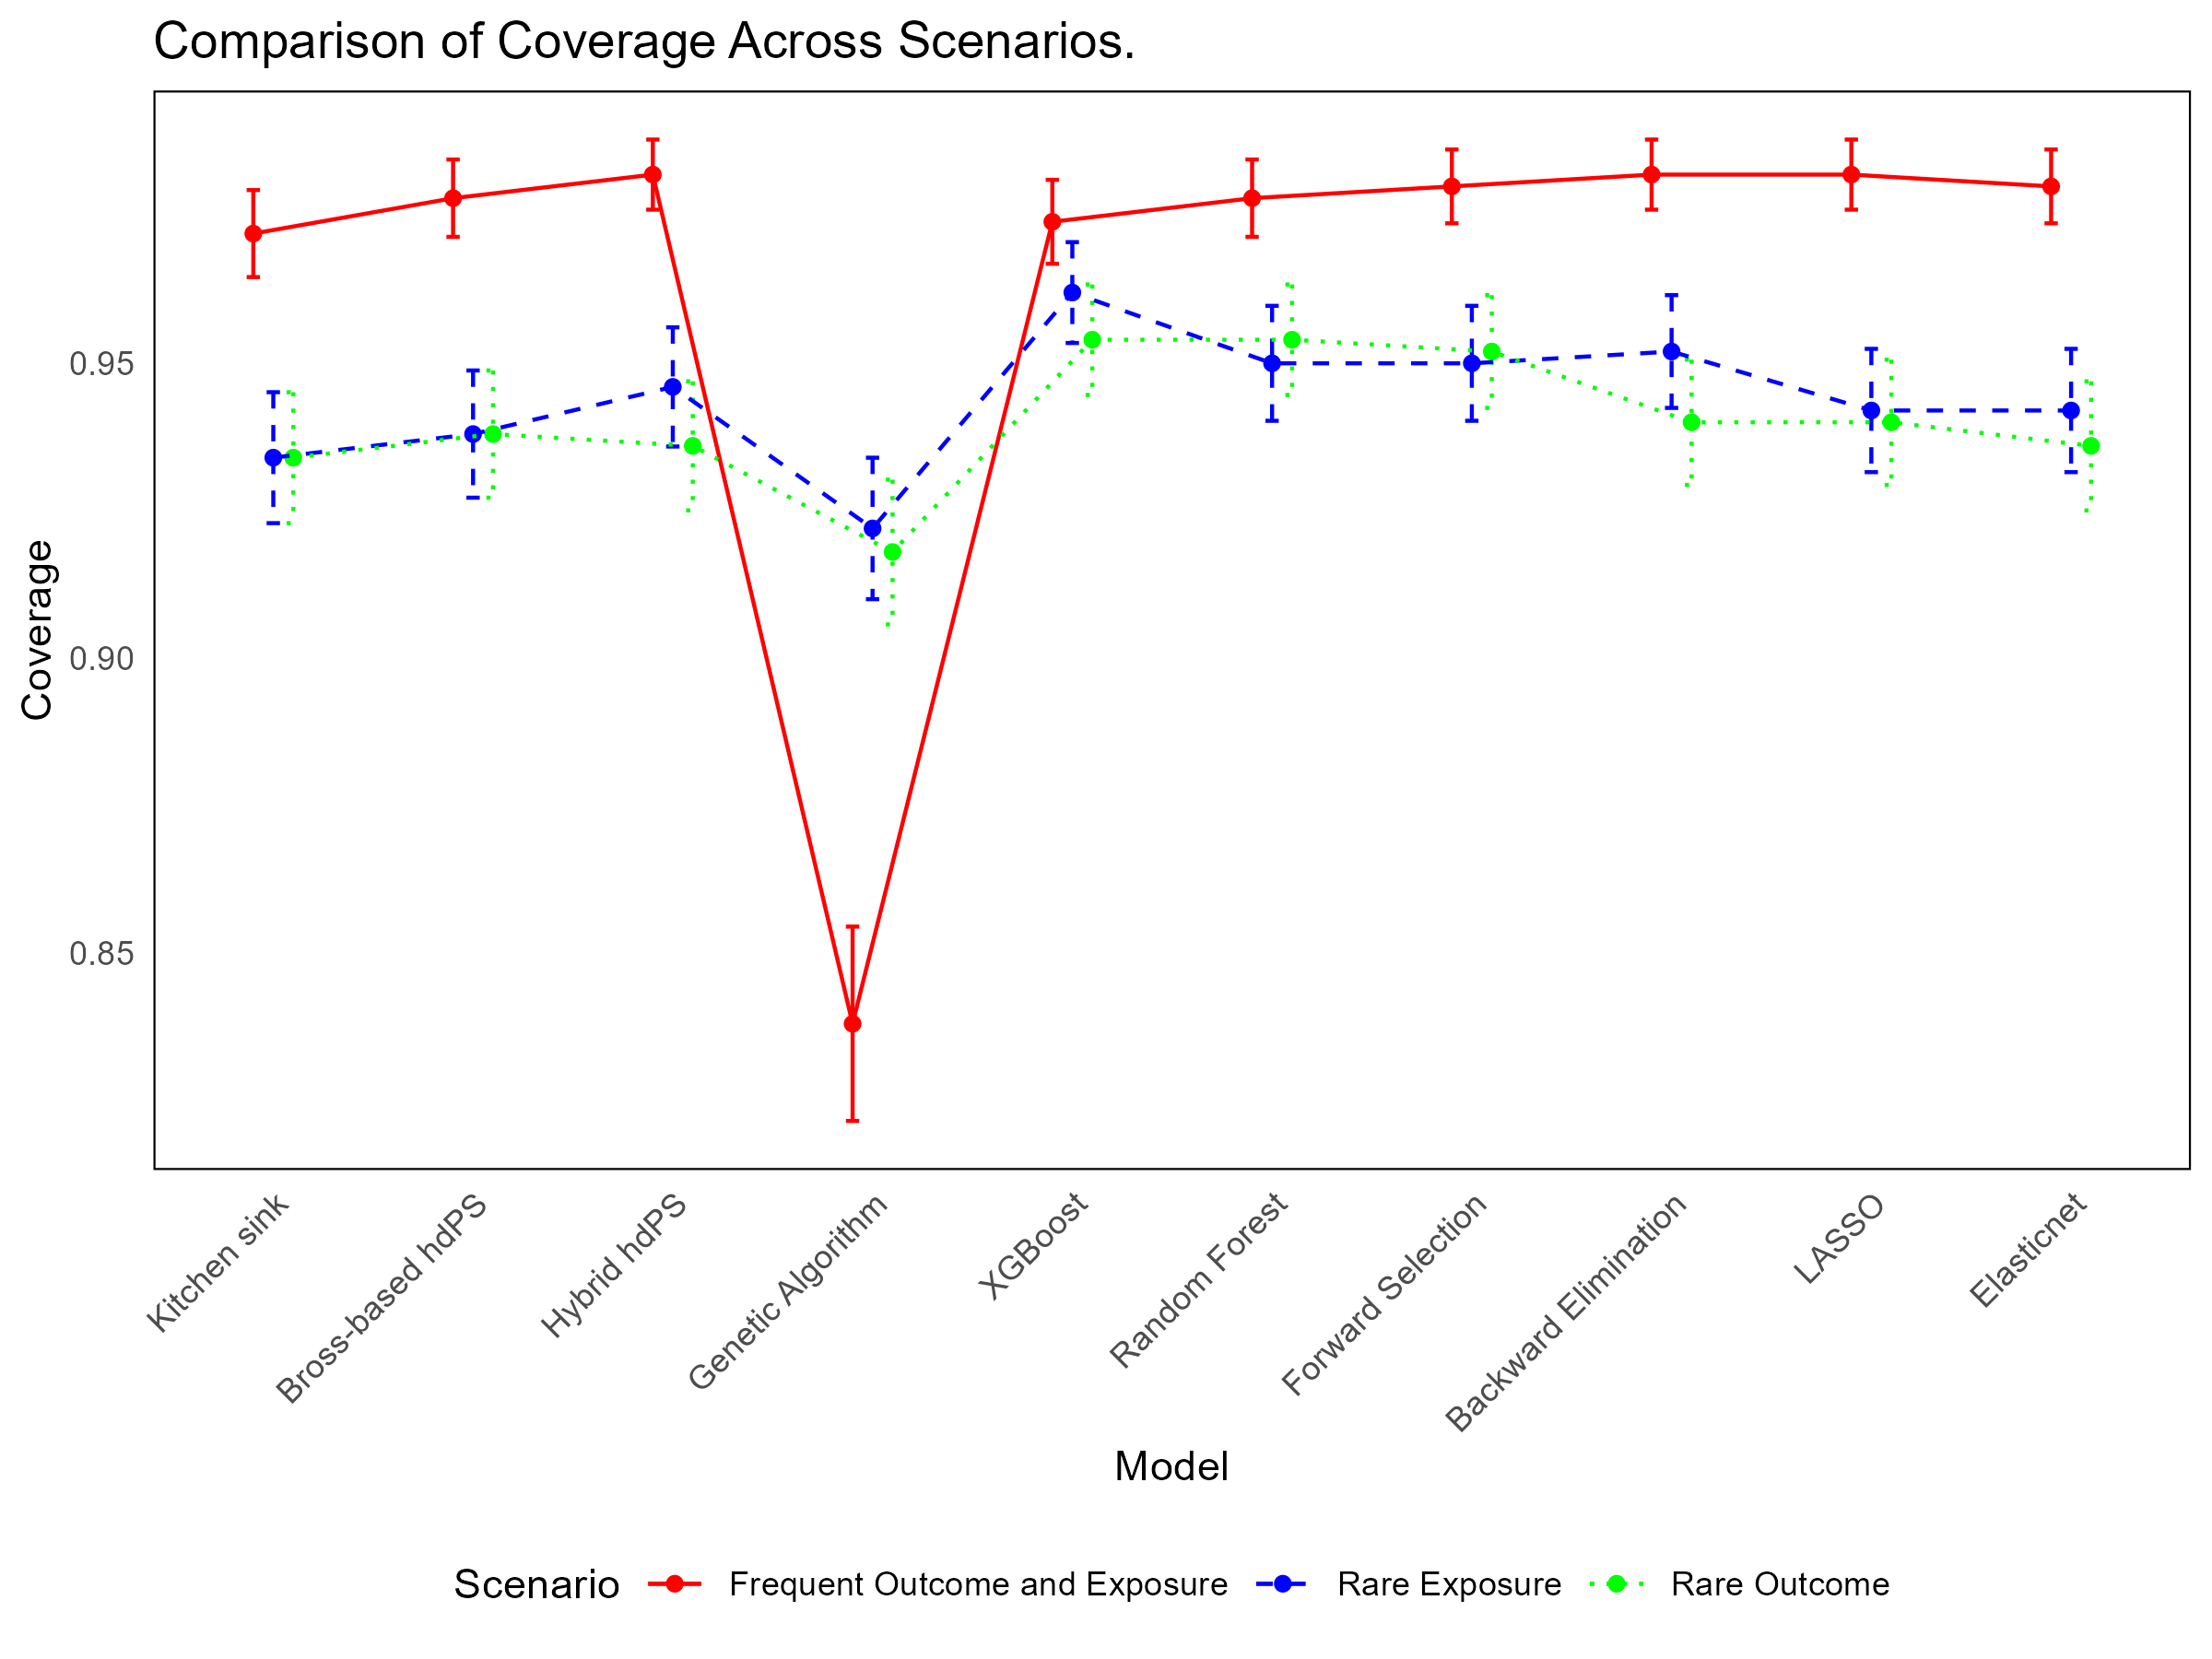
\includegraphics[width=1\linewidth,]{figures/metric_comparison_Coverage} 

}

\caption{Comparison of Coverage Probability Across Different Methods in hdPS Analysis\label{fig:Coverage-comparison}}\label{fig:unnamed-chunk-2}
\end{figure}

\section{Real-world analysis}\label{real-world-analysis}

\emph{Here we include full data analysis (with some summary results like
exposure and outcome prevalence, and sample size) and report OR and RD.
Also mention how many proxies were chosen (add in the picture of RD and
OR; side by side for each method, ordered my magnitude of RD), and how
many were in common with hdPS (add table).}

See Figure \ref{fig:comparison-plot} for the results from analyzing the
NHANES (2013-2018) dataset.

\begin{figure}[th]

{\centering 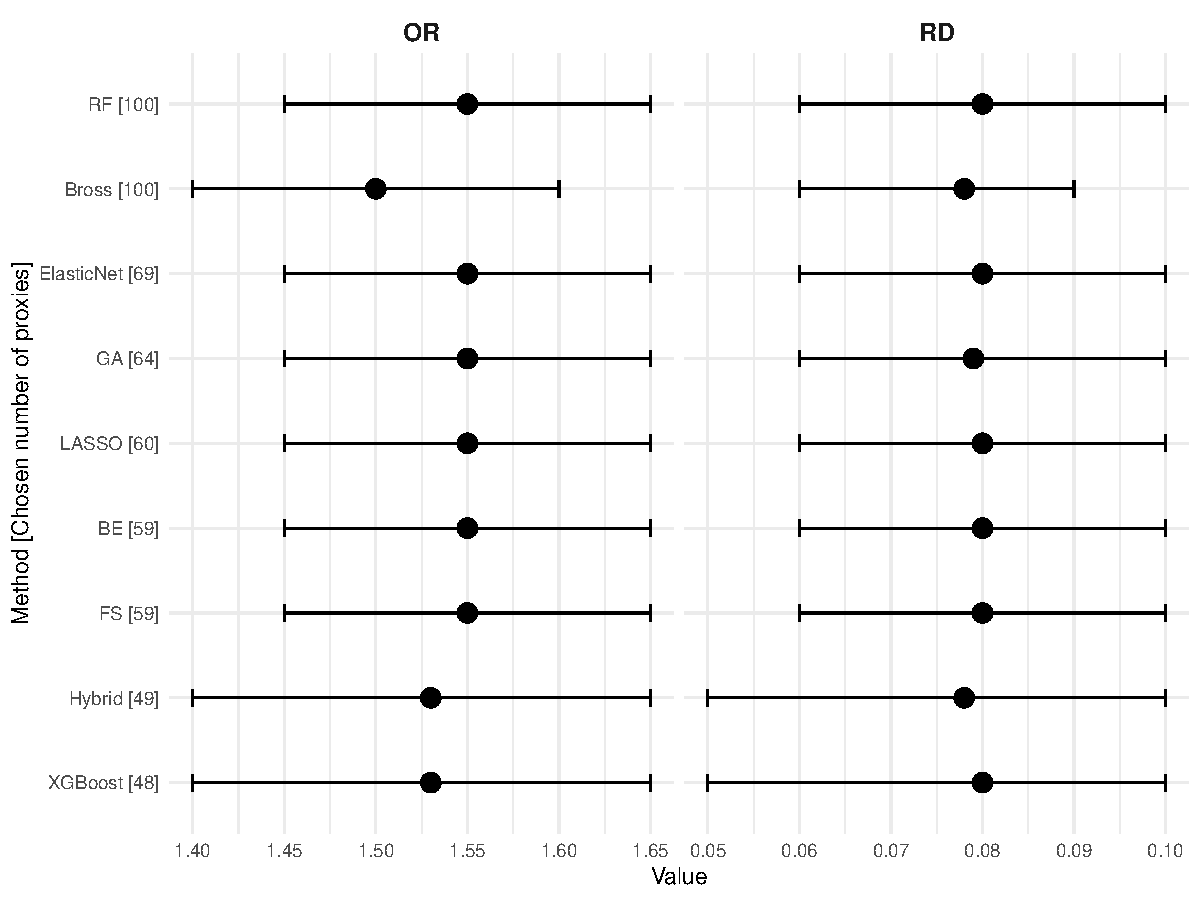
\includegraphics[width=1\linewidth,]{manuscript_files/figure-latex/unnamed-chunk-3-1} 

}

\caption{Figure presenting a comparison of Risk Differences (RD) and Odds Ratios (OR) with 95\% confidence intervals for different methods used to evaluate the association between obesity and diabetes risk. The analysis is based on data from the National Health and Nutrition Examination Survey (NHANES) for the years 2013-2018. Methods are arranged by the number of variables used in the models.\label{fig:comparison-plot}}\label{fig:unnamed-chunk-3}
\end{figure}

Table \ref{tab:method-comparison} presents a pairwise comparison of the
number of proxy features shared between different variable selection
methods used in the analysis. Each cell in the table indicates the count
of common proxy variables selected by the method in the corresponding
row and column. The diagonal cells, where the row and column methods are
the same, represent the total number of proxy variables selected
exclusively by each method.

\begin{table}[htbp]
\centering
\caption{Comparison of variable overlap of selected proxies across different methods used to evaluate the association between obesity and diabetes}
\label{tab:method-comparison}
\begin{tabular}{lccccccccc}
\toprule
 & \textbf{Bross} & \textbf{Hybrid} & \textbf{LASSO} & \textbf{Elasticnet} & \textbf{GA} & \textbf{XGBoost} & \textbf{RF} & \textbf{FS} & \textbf{BE} \\
\midrule
\textbf{Bross formula} & 100 & & & & & & & & \\
\textbf{Hybrid (Bross and LASSO)} & 49 & 49 & & & & & & & \\
\textbf{LASSO} & 47 & 47 & 60 & & & & & & \\
\textbf{Elasticnet} & 54 & 48 & 60 & 69 & & & & & \\
\textbf{Genetic algorithm (GA)} & 44 & 28 & 36 & 40 & 64 & & & & \\
\textbf{XGBoost} & 38 & 24 & 28 & 30 & 25 & 48 & & & \\
\textbf{Random Forest (RF)} & 72 & 37 & 42 & 50 & 36 & 48 & 100 & & \\
\textbf{Forward selection (FS)} & 45 & 41 & 51 & 54 & 35 & 25 & 43 & 59 & \\
\textbf{Backward elimination (BE)} & 45 & 41 & 51 & 54 & 35 & 25 & 43 & 59 & 59 \\
\bottomrule
\end{tabular}
\end{table}

\textbf{Computing time}:

\emph{Report computing time for the Real-world analysis for each method.
(add ordered table)}

\section{Discussion}\label{discussion}

XGBoost consistently outperformed other methods across all scenarios,
demonstrating low bias, high coverage, and the lowest MSE. The GA, on
the other hand, consistently underperformed with higher bias, lower
coverage, and higher MSE, indicating less reliable estimates. The Bross
method and the kitchen sink model generally provided moderate
performance with low to moderate bias and reasonable coverage, but they
were less accurate than XGBoost. Hybrid, Elasticnet, and LASSO methods
showed competitive performance with moderate bias, good coverage, and
acceptable MSE, making them reliable alternatives, though slightly less
optimal than XGBoost.

\textbf{Contextualizing the literature}:

\textbf{Summary of the simulation findings}:

\textbf{Data analysis findings}:

\textbf{Future Direction}:

\textbf{Conclusion}:

\section*{List of abbreviations}\label{list-of-abbreviations}
\addcontentsline{toc}{section}{List of abbreviations}

\begin{itemize}
\tightlist
\item
  hdPS: High-dimensional Propensity Score
\item
  NHANES: National Health and Nutrition Examination Survey
\item
  OR: Odds Ratio
\item
  RD: Risk Difference
\item
  SE: Standard Error
\item
  MSE: Mean Squared Error
\item
  LASSO: Least Absolute Shrinkage and Selection Operator
\item
  GA: Genetic Algorithm
\item
  RF: Random Forest
\item
  XGBoost: Extreme Gradient Boosting
\item
  FS: Forward Selection
\item
  BE: Backward Elimination
\item
  CV: Cross-Validation
\item
  RR: Relative Risk
\item
  Elasticnet: A regularized regression method that combines LASSO and
  Ridge regression
\end{itemize}

\section*{Declarations}\label{declarations}
\addcontentsline{toc}{section}{Declarations}

\subsection*{Ethics approval and consent to
participate}\label{ethics-approval-and-consent-to-participate}
\addcontentsline{toc}{subsection}{Ethics approval and consent to
participate}

The analysis conducted on secondary and de-identified data is exempt
from research ethics approval requirements. Ethics for this study was
covered by item 7.10.3 in University of British Columbia's Policy \#89:
Research and Other Studies Involving Human Subjects 19 and Article 2.2
in of the Tri-Council Policy Statement: Ethical Conduct for Research
Involving Humans (TCPS2).

\subsection*{Consent for publication}\label{consent-for-publication}
\addcontentsline{toc}{subsection}{Consent for publication}

\subsection*{Availability of data and
materials}\label{availability-of-data-and-materials}
\addcontentsline{toc}{subsection}{Availability of data and materials}

\subsection*{Competing interests}\label{competing-interests}
\addcontentsline{toc}{subsection}{Competing interests}

Over the past three years, MEK has received consulting fees from Biogen
Inc.~for consulting unrelated to this current work. MEK was previously
supported by the Michael Smith Foundation for Health Research Scholar
award.

\subsection*{Funding}\label{funding}
\addcontentsline{toc}{subsection}{Funding}

This work was supported by MEK's Natural Sciences and Engineering
Research Council of Canada (NSERC) Discovery Grants and Discovery
Accelerator Supplements.

\subsection*{Authors' contributions}\label{authors-contributions}
\addcontentsline{toc}{subsection}{Authors' contributions}

MEK: Conceptualization, Writing -- Original Draft, Review \& Editing YL:
Formal Analysis, Review \& Editing

\subsection*{Acknowledgements}\label{acknowledgements}
\addcontentsline{toc}{subsection}{Acknowledgements}

Not applicable.

\renewcommand\refname{References}
\bibliography{mergedbibliography.bib}


\end{document}
